\subsection{Akkumulator}
\label{sec:Valid_Batterie}

\subsubsection{ADC Messung der Batteriespannung}

Die Spannungsmessung inkl. Korrekturfaktor für den Spannungsteiler mit Hilfe einer Source Measuring Unit überprüft. Die Dabei entstandenen Werte sind in der Abbildung \ref{pic:ADC_Spannung_Graph} geplottet.

\begin{figure}[H]
	\centering
	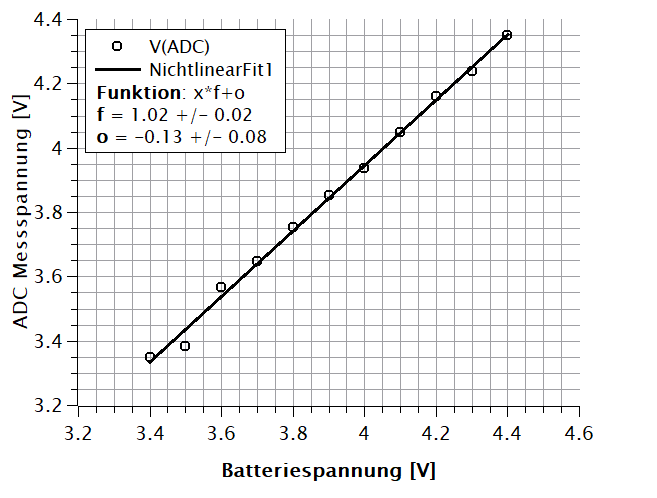
\includegraphics[width=0.8\linewidth]{ADC_Spannung_Graph}
	\caption{Akkumulatorspannung im Vergleich mit der gemessenen Spannung am ADC}
	\label{pic:ADC_Spannung_Graph}
\end{figure}

Auf die gemessenen Werte liefert ein linearer Fit folgende Erkenntnis.
Die Messwerte sind durchschnittlich um $V_{offset}=-130\si{mV}$ zu gering.
Zu einem Teil sind die Abweichungen auf die Widerstandtoleranzen des Spannungsteilers zurückzuführen.
Ein weiterer Einflussfaktor hat die Batteriespannung selber, da diese durch den BQ2409x nicht konstant gehalten wird. Auch das Fehlen einer Filterschaltung für das ADC Signal verschlechtert die Messergebnisse.

Verwendetes Messgerät:

Agilent N6705B (Prüfmittel Nr. \texttt{MSZ-M-0064}) auf Channel 1 mit Strombegrenzung $I_{max}=600\si{mA}$.



